\documentclass[a4paper,10pt]{article}
%\documentclass[a4paper,10pt]{scrartcl}
\usepackage[spanish]{babel}
\usepackage[utf8]{inputenc}
\usepackage{amssymb, amsmath, amsbsy}
\usepackage{cancel} % para tachar
\usepackage{mathdots} % para el comando \iddots
\usepackage{mathrsfs} % para formato de letra
\usepackage{stackrel} % para el comando \stackbin
\usepackage{graphicx}
\graphicspath{ {images/} }

\title{\begin{center}

\includegraphics[width=\textwidth]{logoupzmg.png}
\end{center}
Practica 6 \\ Analisis de elementos finitos al robot}
\author{Alvarado Galicia Felipe \\
Gutiérrez Muñoz José de Jesús \\ 
Medina Rodríguez Francisco Javier \\
Martínez Noyola Moisés Emanuel \\ 
Pasillas Gonzáles Iván Pasillas \\ 
7 - A \\ 
Ing. Mecatrónica}
\date{2 - Noviembre - 2019}

\break

\begin{document}
\maketitle

\break

\tableofcontents

\chapter{Definición}

\hfill

\chapter{Aplicaciones}

\hfill

\chapter{Análisis por elementos finitos}

\hfill

\chapter{Pre-procesamiento}

\hfill

\chapter{Análisis (cómputo de la solución)}

\hfill

\chapter{Post-procesamiento (visualización)}

\hfill

\chapter{Desarrollo}

\hfill

\chapter{Selección del material}

\break

\textbf{Definición.}

\hfill

El análisis por elementos finitos (FEA, siglas en inglés de Finite Element Analysis) es una técnica de simulación por computador usada en ingeniería. Usa una técnica numérica llamada método de los elementos finitos (FEM).

Existen muchos paquetes de software, tanto libres como no libres. El desarrollo de elementos finitos en estructuras, suele basarse en análisis energéticos como el principio de los trabajos virtuales.

\hfill

\textbf{Aplicaciones.}

\hfill

En estas aplicaciones, el objeto o sistema se representa por un modelo geométricamente similar que consta de múltiples regiones discretas simplificadas y conectadas. Ecuaciones de equilibrio, junto con consideraciones físicas aplicables, así como relaciones constitutivas, se aplican a cada elemento, y se construye un sistema de varias ecuaciones. El sistema de ecuaciones se resuelve para los valores desconocidos usando técnicas de álgebra lineal o esquemas no lineales, dependiendo del problema. Siendo un método aproximado, la precisión de los métodos FEA puede ser mejorada refinando la discretización en el modelo, usando más elementos y nodos.

Comúnmente se usa FEA en determinar los esfuerzos y desplazamientos en sistemas mecánicos. Es además usado de manera rutinaria en el análisis de muchos otros tipos de problemas, entre ellos Transferencia de calor, dinámica de fluidos, y electromagnetismo. Con FEA se pueden manejar sistemas complejos cuyas soluciones analíticas son difícilmente calculables.

\hfill

\textbf{Análisis por elementos finitos.}

\hfill

En general, hay tres fases en cualquier tarea asistida por computador:

\begin{itemize}
 \item Pre-procesamiento. Definir el modelo de elementos finitos y los factores ambientales que influyen en él.
 \item Solución del análisis. Solucionar el modelo de elementos finitos.
 \item Post-procesamiento de resultados usando herramientas de visualización.
\end{itemize}

\hfill

\textbf{Pre-procesamiento.}

\hfill

El primer paso en FEA, pre-procesamiento, es construir un modelo de elementos finitos de la estructura a ser analizada. En muchos paquetes de FEA se requiere de la entrada de una descripción topológica de las características geométricas de la estructura.3​ Ésta puede ser 1D, 2D, o 3D. El objetivo principal del modelo es replicar de manera realista los parámetros importantes y características del modelo real.3​ La manera más sencilla para conseguir similaridad en el análisis es utilizar planos pre existentes, modelos CAD, o datos importados de un ambiente FEA. Una vez se ha creado la geometría, se utiliza un procedimiento para definir y dividir el modelo en "pequeños" elementos. En general, un modelo de elementos finitos está definido por una malla, la cual está conformada por elementos y nodos. Los nodos representan puntos en los cuales se calcula el desplazamiento (análisis estructural). Los paquetes de FEA enumeran los nodos como una herramienta de identificación. Los elementos están determinados por conjuntos de nodos, y definen propiedades localizadas de masa y rigidez. Los elementos también están definidos por la numeración de la malla, la cual permite referenciar la correspondiente deflexión o esfuerzo (en análisis estructural) para una localización específica.

\hfill

\textbf{Análisis (cómputo de la solución).}

\hfill

En la siguiente etapa en el proceso de análisis de elementos finitos se lleva a cabo una serie de procesos computacionales que involucran fuerzas aplicadas, y las propiedades de los elementos de donde producir un modelo de solución. Tal análisis estructural permite la determinación de efectos como lo son las deformaciones, estiramiento o estrés que son causados por fuerzas estructurales aplicadas como lo son la fuerza, la presión y la gravedad.

\hfill

\textbf{Post-procesamiento (visualización).}

\hfill

Estos resultados entonces pueden ser estudiados utilizando herramientas visuales dentro del ambiente de FEA para ver y para identificar completamente las implicaciones del análisis. Herramientas numéricas y gráficas permiten la localización precisa de información como esfuerzos y deformaciones a ser identificadas.

\hfill

\textbf{Desarrollo.}

\hfill

Simulación del análisis de tensión al robot.

\begin{center}
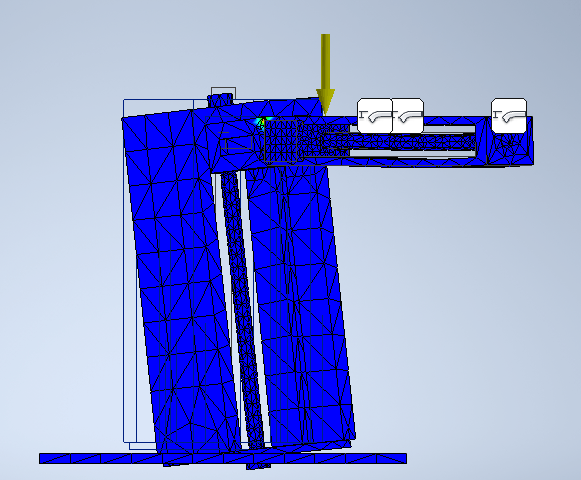
\includegraphics[width=\textwidth]{Tension1.png}
Figura 1. Simulación: Aplicación de fuerza en el ultimo eslabón.
\end{center}

\begin{center}
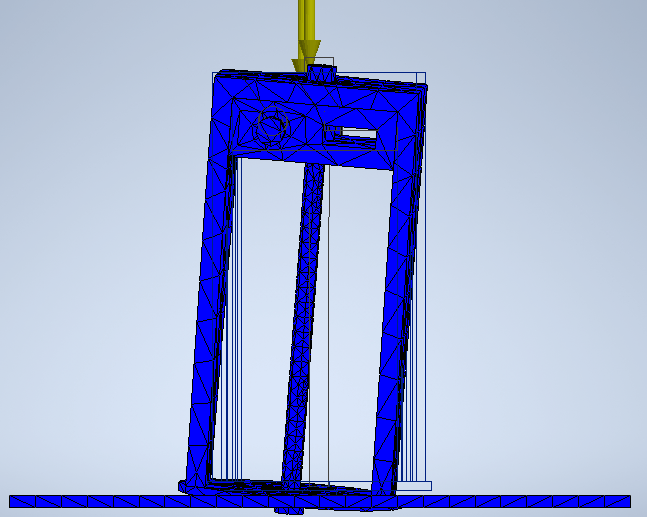
\includegraphics[width=\textwidth]{Tension2.png}
Figura 2. Vista frontal de la simulación.
\end{center}

\begin{center}
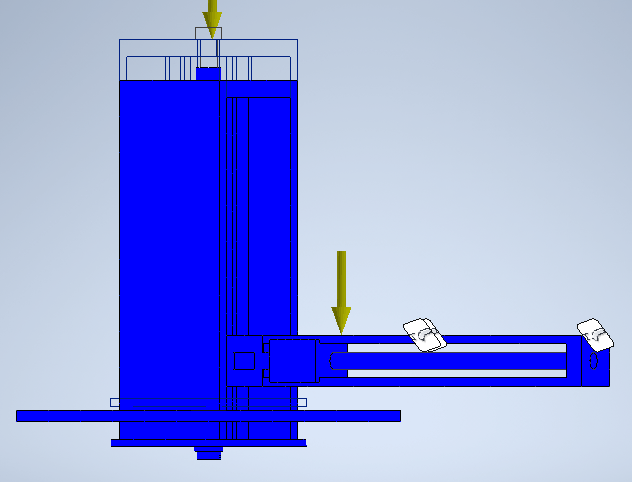
\includegraphics[width=\textwidth]{Tension3.png}
Figura 3. Aplicación de fuerza con el elemento móvil en el punto más bajo.
\end{center}

\begin{center}
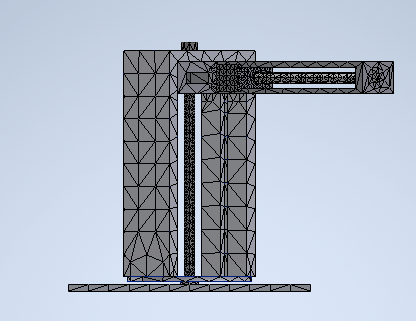
\includegraphics[width=\textwidth]{vistamalla.png}
Figura 4. Mallas en el robot.
\end{center}

\break

\textbf{Selección del material.}

\hfill

Debido al uso para el que estará destinado el robot se llegó a la conclusión de utilizar aluminio para la estructura principal.

Beneficios del aluminio.

El aluminio es ligero, con una densidad de un tercio de la del acero: 2,700 kg/m3. 

El aluminio presenta una resistencia a la tracción de entre 70 a 700 MPa dependiendo de la aleación y del proceso de elaboración. Los perles extruidos de aluminio con una aleación y un diseño apropiados pueden llegar a ser tan resistentes como el acero estructural.

El módulo de elasticidad (módulo de Young) del aluminio es un tercio que el del acero (E=70.000 MPa). Esto significa que el momento de inercia debe ser tres veces mayor en una extrusión de aluminio para lograr la misma deflexión que un perfil de acero.

El aluminio posee una facilidad de conformado óptima, una característica que se aprovecha al máximo en la extrusión. El aluminio también se puede soldar, curvar, estirar, punzonar y fresar.

Reciclaje: El aluminio es un material con muy buenas propiedades de reciclado. Sólo el 5 por ciento de la energía requerida para producir el metal primario inicialmente es requerida para volverlo a fundir, manteniéndose las propiedades del metal durante el proceso.

\end{document}
